\documentclass[11pt,letterpaper]{article}

\usepackage{amsmath}
\usepackage{amssymb}
\usepackage{fancyhdr}
\usepackage{verbatim}
\usepackage{graphicx}


\oddsidemargin0cm
\topmargin-2cm
\textwidth16.5cm
\textheight23.5cm

\newcommand{\question}[1] {\vspace{.25in} \hrule\vspace{0.5em}
\noindent{\bf #1} \vspace{0.5em}
\hrule \vspace{.10in}}
\renewcommand{\part}[1] {\vspace{.10in} {\bf (#1)}}

\newcommand{\myname}{Karan Sikka}
\newcommand{\myandrew}{ksikka@cmu.edu}
\newcommand{\myhwnum}{03}

\setlength{\parindent}{0pt}
\setlength{\parskip}{5pt plus 1pt}

\pagestyle{fancyplain}
\lhead{\fancyplain{}{\textbf{PS\myhwnum}}}
\rhead{\fancyplain{}{\myname\\ \myandrew}}
\chead{\fancyplain{}{02-512}}

\begin{document}

\medskip

\thispagestyle{plain}
\begin{center}                  % Center the following lines
{\Large 02-512 Assignment \myhwnum} \\
\myname \\
\myandrew \\
\today
\end{center}

\question{1}

\part{a}

For some protein $p$, the state set is
\texttt{folded},
\texttt{unfolded}, or
\texttt{misfolded}.

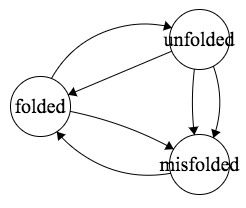
\includegraphics[scale=0.6]{1a}

\part{b}

For some proteins $p1,p2$, the state set is
\texttt{unfolded,unfolded},
\texttt{unfolded,folded},
\texttt{unfolded,misfolded},
\texttt{folded,misfolded},
\texttt{folded,misfolded}, or
\texttt{misfolded,misfolded}.

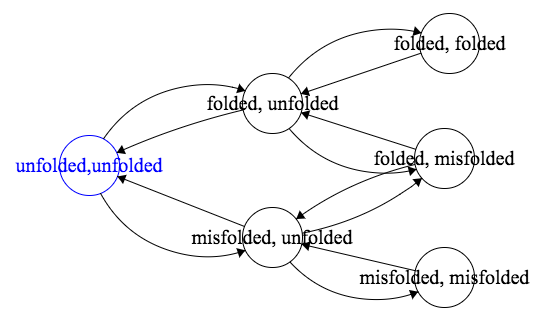
\includegraphics[scale=0.6]{1b}

\part{c}

\question{2}
\part{a}

\part{b}

\part{c}

\part{d}

\part{e}

\question{3}
\part{a}

\part{b}

\part{c}

\part{d}

\question{4}

\part{a}

\part{b}

\part{c}

\part{d}

\part{e}


\end{document}
